\FloatBarrier

{\color{red} 

\section{Comparison Between VALOR and P-theta Results using Full Run 1-9 Statistics} \label{app:compare_valor_ptheta}

To validate the results of this analysis, they are compared to the results obtained by the P-theta group. The P-theta analysis \cite{PthetaR19cNuebarAppearance} uses electron-like spectra binned in $(p, \theta)$ variables, while the VALOR analysis uses $(E_{\text{rec}}, \theta)$. The use of different binning variables will cause the calculation of the control sample likelihood weights (in both rate-only and rate+shape analyses) and marginal likelihood to be different between VALOR and P-theta. Therefore the p-values in the P-theta tech note (see ref \cite{PthetaR19cNuebarAppearance}) are not directly comparable to the p-values in this document. Instead the P-theta group has duplicated their rate+shape analyses using $(E_{\text{rec}}, \theta)$ binning to produce the p-values which are considered in this section.


\subsection{Comparison of Expected Sensitivities}\label{app:compare_sensitivity_valor_ptheta}

The P-theta analysis was completed before the Asimov A true value of $\sin^{2} 2 \theta_{13}$ was updated to 0.0830, so used the previous value of 0.0856. In order to have directly comparable p-values, the VALOR p-values shown in this section were produced using the same value of $\sin^{2} 2 \theta_{13}$ as used in the P-theta analysis, so are not the same p-values shown in section \ref{sec:run1-9d_sensitivity}.

For the rate-only analysis, VALOR expects a test statistic of 17.13 events, while P-theta expects 17.15 events. For the rate+shape analysis, VALOR expects a test statistic of $\Delta \chi^2 = 6.73$, while P-theta expects $\Delta \chi^2 = 6.69$. Figs \ref{fig:sensitivity_rate-only_valor_vs_ptheta} and \ref{fig:sensitivity_rate+shape_valor_vs_ptheta} show the expected rate-only and rate+shape test statistic distributions. As Tab \ref{tab:compare_pvals_sensitivity_valor_ptheta} shows, the p-values produced by VALOR and P-theta are in good agreement.

\begin{table}[H]
\centering
\begin{tabular}{|c|c|c|c|c|}
	\hline
	Analysis                    & Fake data $\beta$   & Group                   & p-value              & $\sigma$                \\
	\hline
	
	
	\multirow{4}{*}{rate-only}  & \multirow{ 2}{*}{0} & VALOR                   & $0.0102 \pm 0.0007$  & $2.57 \pm 0.02$         \\
	\cline{3-5}
	                            &                     & P-theta                 & $0.0109$             & $2.55$                  \\
	\cline{2-5}
	                            & \multirow{ 2}{*}{1} & VALOR                   & $0.465 \pm 0.004$    & $0.73 \pm 0.01$         \\
	\cline{3-5}
	                            &                     & P-theta                 & $0.453$              & $0.75$                  \\
	\hline
	
	
	\multirow{4}{*}{rate+shape} & \multirow{ 2}{*}{0} & VALOR                   & $0.0046 \pm 0.0005$  & $2.83^{+0.04}_{-0.03}$  \\
	\cline{3-5}
	                            &                     & P-theta                 & 0.00369              & 2.90                    \\
	\cline{2-5}
	                            & \multirow{ 2}{*}{1} & VALOR                   & $0.439 \pm 0.004$    & $0.77 \pm 0.01$         \\
	\cline{3-5}
	                            &                     & P-theta                 & 0.429                & 0.79                    \\
	\hline
	
	
\end{tabular}
\caption{
	Comparison of the p-values given by the Asimov A sensitivity studies from the VALOR and P-theta groups.
}
\label{tab:compare_pvals_sensitivity_valor_ptheta}
\end{table}





\subsection{Comparison of Data Results} \label{app:compare_data_valor_ptheta}

For the rate-only analysis the observed test statistic, the event rate in the antineutrino mode single-ring e-like sample (\NskObservedNueBarRunOneNineD\ events) is the same for VALOR and P-theta, as expected. For the rate+shape analysis, differences in the ensemble of marginalisation toys causes slightly different observed $\Delta \chi^2$ values, 3.81 for VALOR and 4.09 for P-theta. Figs \ref{fig:data_rate-only_valor_vs_ptheta} and \ref{fig:data_rate+shape_valor_vs_ptheta} show the observed rate-only and rate+shape test statistic distributions. As Tab \ref{tab:compare_pvals_data_valor_ptheta} shows, the p-values produced by VALOR and P-theta are in good agreement, with the exception of the rate-only $\beta = 1$ p-value. This discrepancy is thought to be due to the fact that for the rate-only analysis, the P-theta group has only used $(p, \theta)$ binning to calculate the control sample likelihood weights (see appendix \ref{app:sampling_vs_reweighting}), and an equivalent rate-only analysis using $(E_{\text{rec}}, \theta)$ binning is not available. This difference is not seen in the rate-only sensitivity study, similarly to the Run 1-9 joint analysis \cite{OurRun19JointAnalysis3Flavour}, where differences in the oscillation parameter confidence intervals produced by VALOR and P-theta are seen in the data fits but not in the sensitivity study.



\begin{table}[H]
\centering
\begin{tabular}{|c|c|c|c|c|}
	\hline
	Analysis                    & Fake data $\beta$   & Group                   & p-value              & $\sigma$                \\
	\hline
	
	
	\multirow{4}{*}{rate-only}  & \multirow{ 2}{*}{0} & VALOR                   & $0.059 \pm 0.002$    & $1.89^{+0.02}_{-0.01}$  \\
	\cline{3-5}
	                            &                     & P-theta                 & 0.0686               & 1.82                    \\
	\cline{2-5}
	                            & \multirow{ 2}{*}{1} & VALOR                   & $0.321 \pm 0.003$    & $0.99 \pm 0.01$         \\
	\cline{3-5}
	                            &                     & P-theta                 & 0.246                & 1.16                    \\
	\hline
	
	
	\multirow{4}{*}{rate+shape} & \multirow{ 2}{*}{0} & VALOR                   & $0.0163 \pm 0.0009$  & $2.40 \pm 0.02$         \\
	\cline{3-5}
	                            &                     & P-theta                 & 0.0155               & 2.42                    \\
	\cline{2-5}
	                            & \multirow{ 2}{*}{1} & VALOR                   & $0.300 \pm 0.004$    & $1.04 \pm 0.01$         \\
	\cline{3-5}
	                            &                     & P-theta                 & 0.300                & 1.04                    \\
	\hline
	
	
\end{tabular}
\caption{
	Comparison of the observed p-values from the VALOR and P-theta groups.
}
\label{tab:compare_pvals_data_valor_ptheta}
\end{table}



\FloatBarrier

\begin{figure}
	\centering
	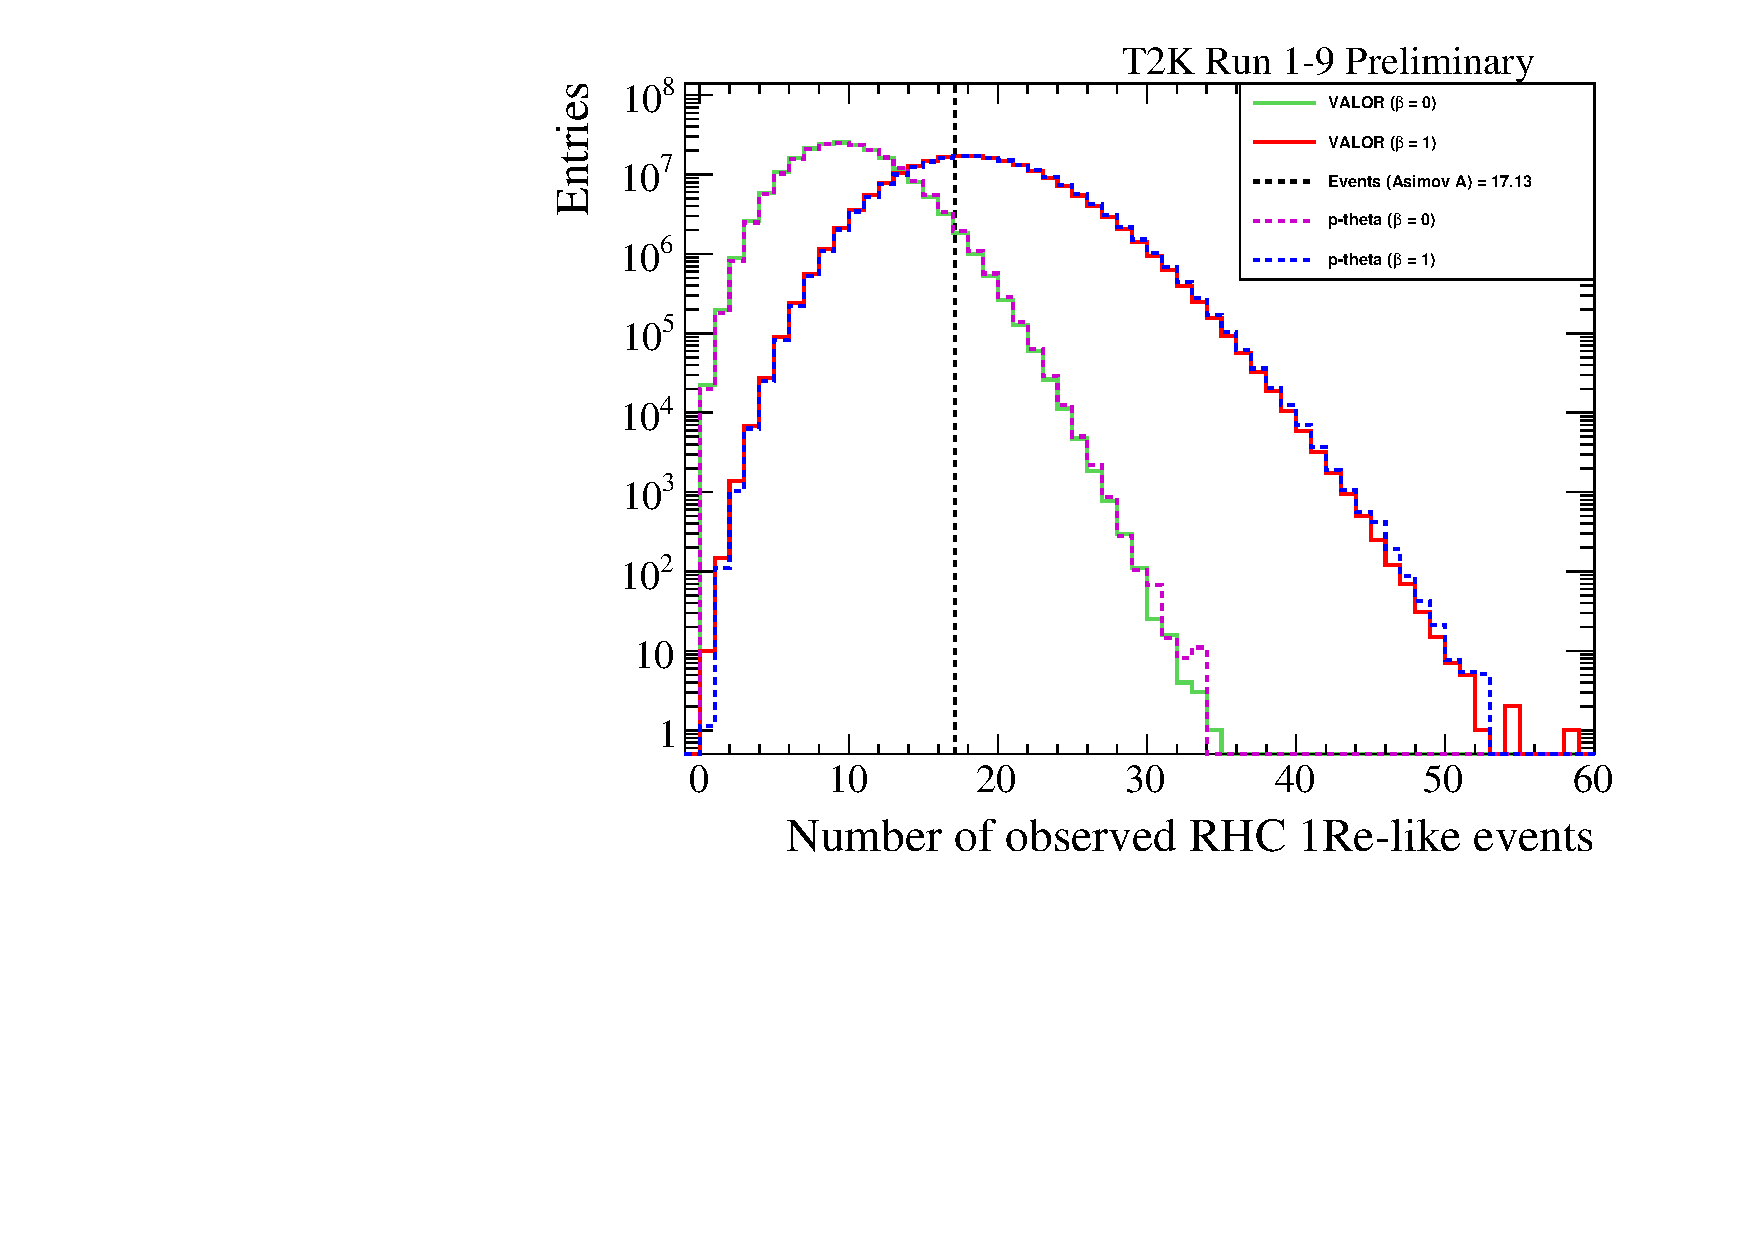
\includegraphics[scale=0.65]{sensitivity/compare_valor_ptheta_R1-9d/nuebarapp_graphs_nmargtoys=200k_nexp=20k_rate-only_MCsampling_VALOR_vs_ptheta_logscale_comparison_nevents}
	
	\caption{Comparison between the expected VALOR and P-theta distributions of the total number of events in the antineutrino mode single-ring e-like sample. The VALOR distributions were produced with \NToysFakeDataRateOnly\ toy experiments using MC sampling (see appendix \ref{app:sampling_vs_reweighting}). The P-theta distributions were produced with 100k toy experiments using re-weighting. Asimov A spectra were used to calculate the 4-sample likelihood.}
	
	\label{fig:sensitivity_rate-only_valor_vs_ptheta}
\end{figure}

\begin{figure}
	\centering
	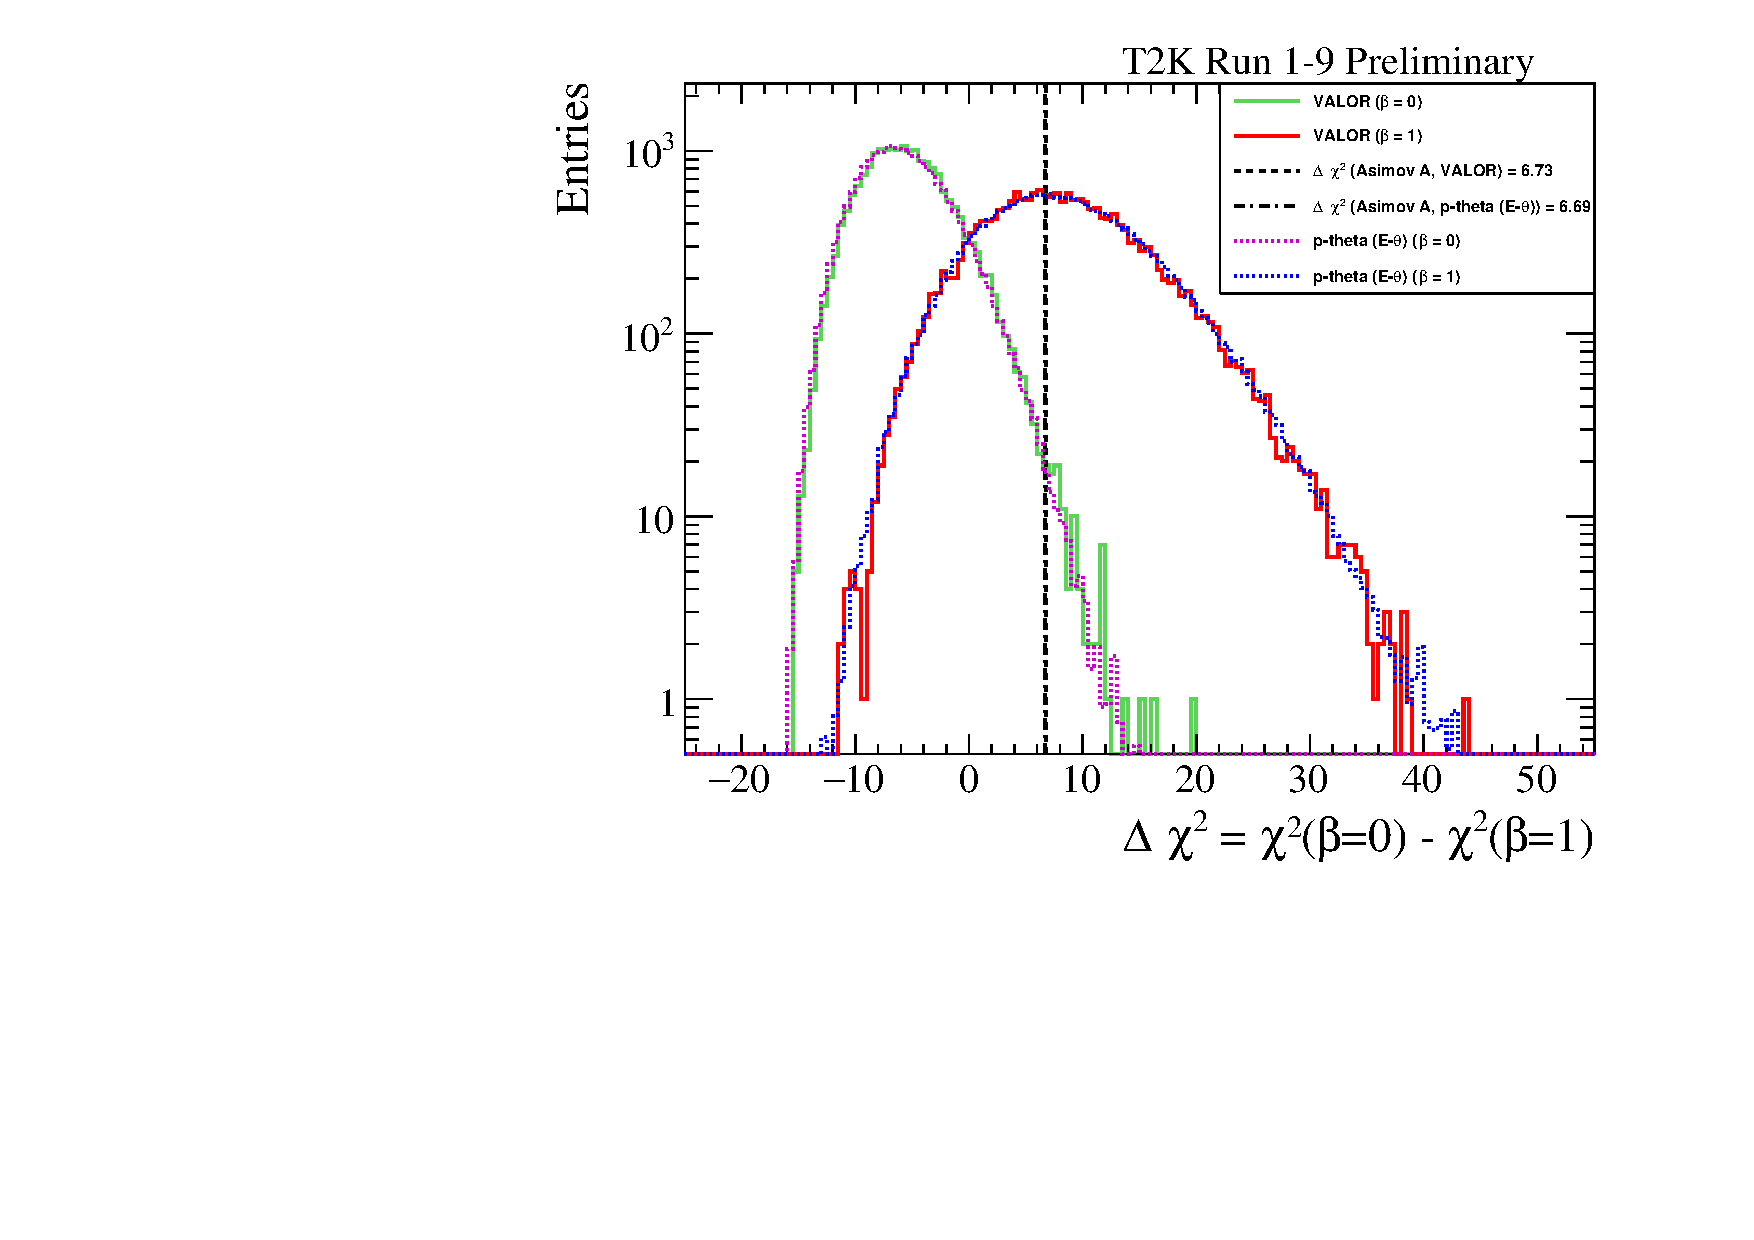
\includegraphics[scale=0.65]{sensitivity/compare_valor_ptheta_R1-9d/nuebarapp_graphs_nmargtoys=200k_nexp=20k_rate+shape_method2_MCsampling_VALOR_vs_ptheta_etheta_logscale_comparison_Deltachisq}
	
	\caption{Comparison between the expected VALOR and P-theta $\Delta \chi^2$ distributions. The VALOR distributions were produced with \NToysFakeDataRateOnly\ toy experiments using MC sampling (see appendix \ref{app:sampling_vs_reweighting}). The P-theta distributions were produced with 2000k toy experiments using re-weighting. Asimov A spectra were used to calculate the 4-sample likelihood.}
	
	\label{fig:sensitivity_rate+shape_valor_vs_ptheta}
\end{figure}



\begin{figure}
	\centering
	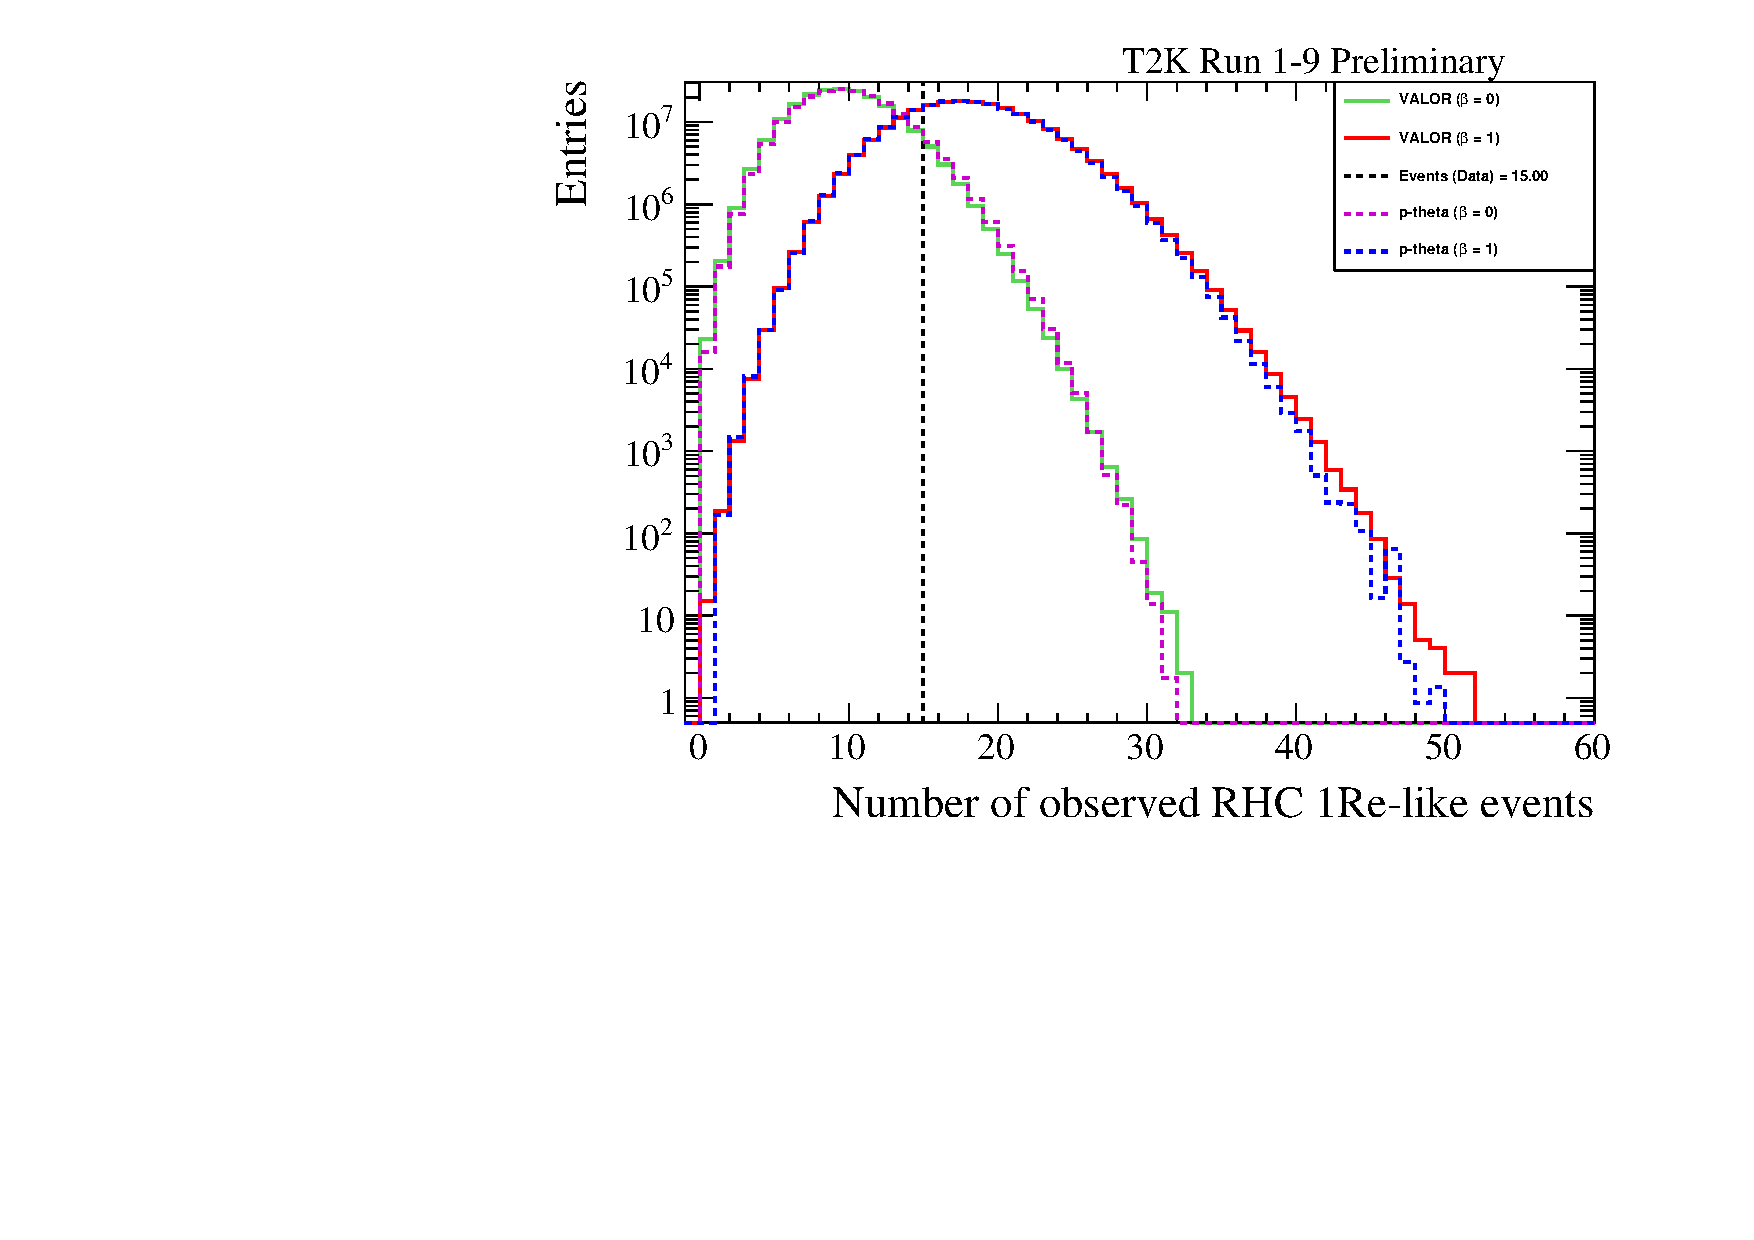
\includegraphics[scale=0.65]{data/compare_valor_ptheta_R1-9d/nuebarapp_graphs_nmargtoys=200k_nexp=20k_data_rate-only_MCsampling_VALOR_vs_ptheta_comparison_nevents_log}
	
	\caption{Comparison between the observed VALOR and P-theta distributions of the total number of events in the antineutrino mode single-ring e-like sample. The VALOR distributions were produced with \NToysFakeDataRateOnly\ toy experiments using MC sampling (see appendix \ref{app:sampling_vs_reweighting}). The P-theta distributions were produced with 100k toy experiments using re-weighting. Observed Run 1-9 spectra were used to calculate the 4-sample likelihood.}
	
	\label{fig:data_rate-only_valor_vs_ptheta}
\end{figure}

\begin{figure}
	\centering
	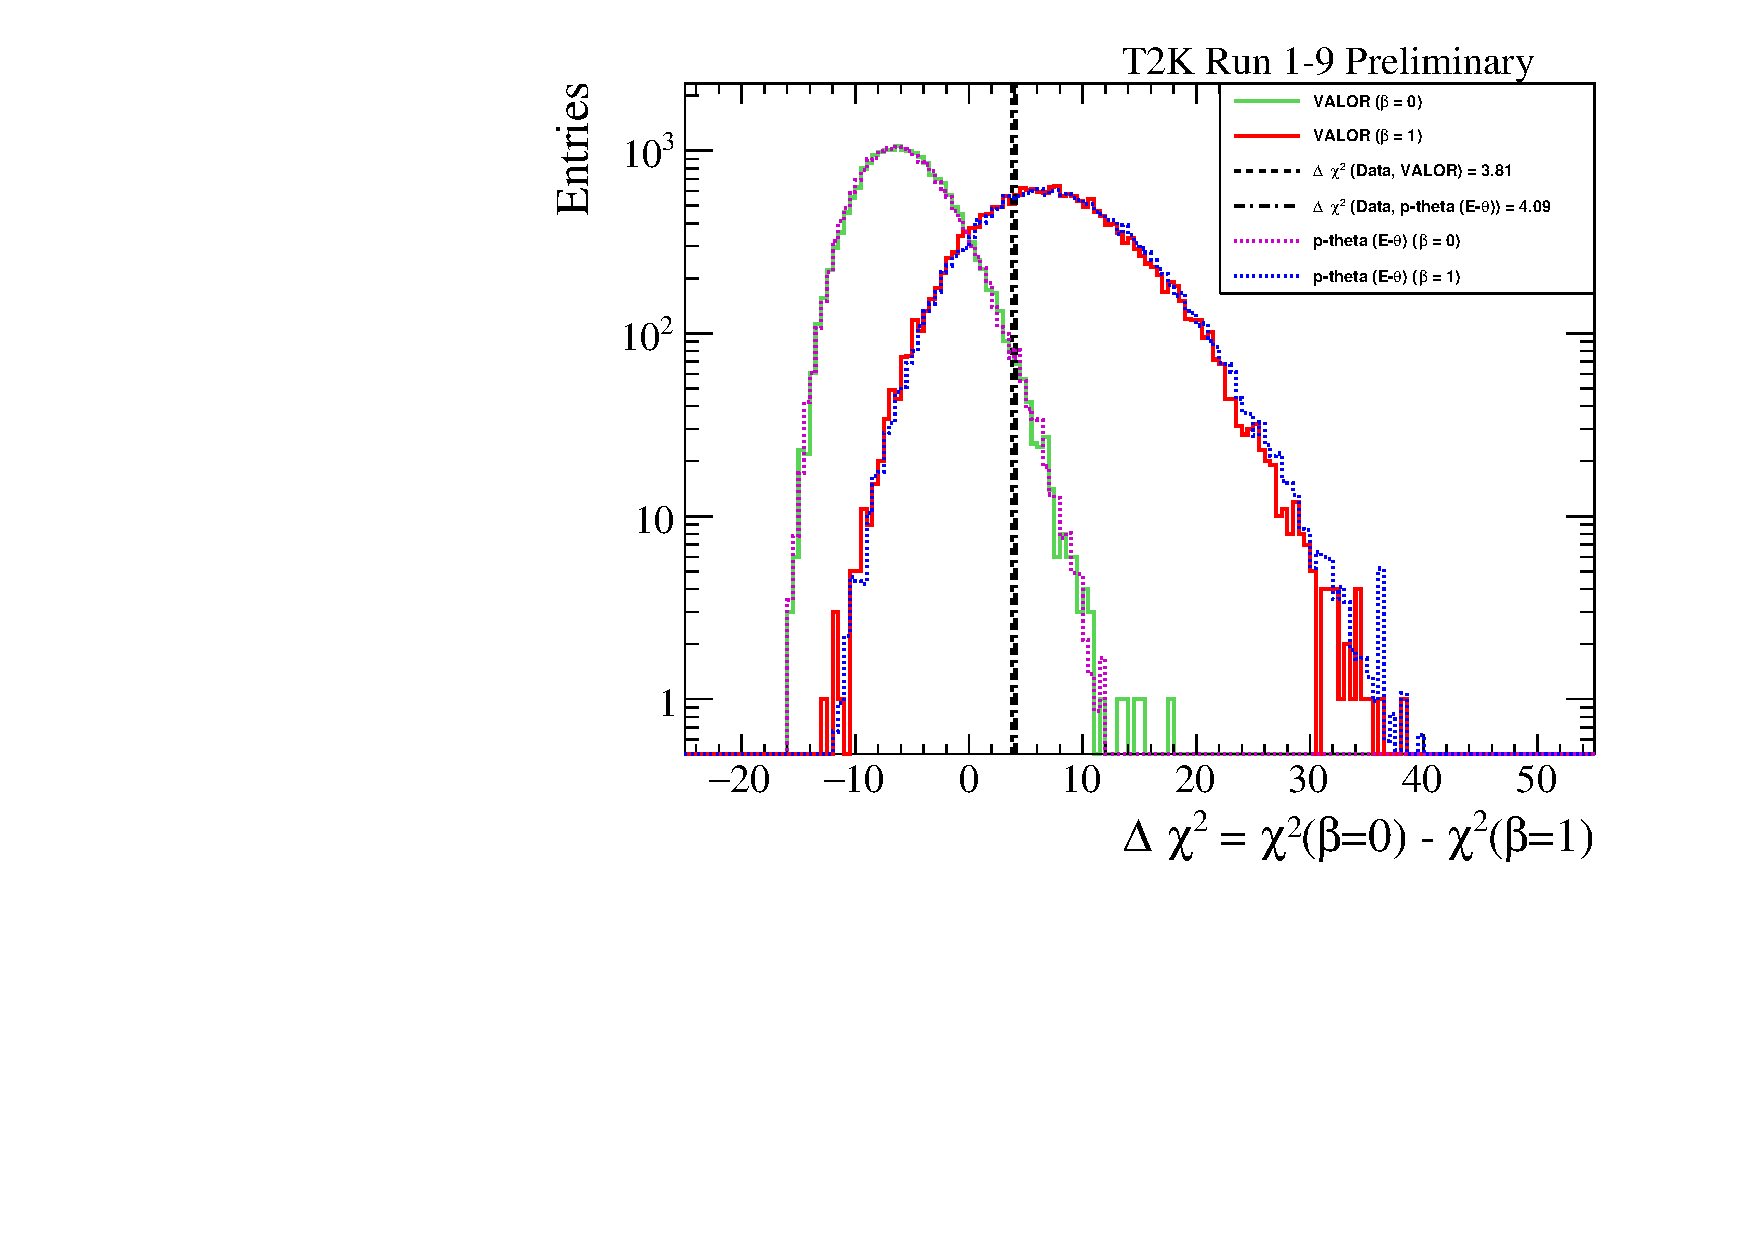
\includegraphics[scale=0.65]{data/compare_valor_ptheta_R1-9d/nuebarapp_graphs_nmargtoys=200k_nexp=20k_data_rate+shape_method2_MCsampling_VALOR_vs_ptheta_etheta_logscale_comparison_Deltachisq}
	
	\caption{Comparison between the observed VALOR and P-theta $\Delta \chi^2$ distributions. The VALOR distributions were produced with \NToysFakeDataRateOnly\ toy experiments using MC sampling (see appendix \ref{app:sampling_vs_reweighting}). The P-theta distributions were produced with 2000k toy experiments using re-weighting. Observed Run 1-9 spectra were used to calculate the 4-sample likelihood.}
	
	\label{fig:data_rate+shape_valor_vs_ptheta}
\end{figure}

} % \colour{red}

\FloatBarrier